\documentclass[../../../main.tex]{subfiles}
\begin{document}
\subsection*{Electric Field}
\subsubsection*{Coulomb's Law.} The force on a test charge $Q$ due to a single point charge $q$ is given by Coulomb's law
\begin{equation*}
    \mathbf{F}=\frac{1}{4\pi \epsilon_0}\frac{q\;Q}{\rcurs^2}\hrcurs
\end{equation*}
The constant $\epsilon_0$ is called (ludicrously) the permittivity of free space. In SI units, where force is in newtons (N), distance in meters (m), and charge in coulombs (C),
\begin{equation*}
    \epsilon_0=8.85\times 10^{-12}\frac{\text{C$^2$}}{\text{Nm$^2$}}
\end{equation*}

\subsubsection*{Electric Field.} Total force on Q can be written as 
\begin{equation*}
    \mathbf{F}=Q\mathbf{E}
\end{equation*}
where
\begin{equation*}
    \mathbf{E}=\frac{1}{4\pi \epsilon_0}\sum_{i=1}^{n}\frac{q_i}{\rcurs_i^2}\hrcurs
\end{equation*}

\subsubsection*{Continuous Charge Distributions.} 
If, instead, the charge is distributed continuously over some region, the sum becomes an integral 
\begin{equation*}
    \mathbf{E}=\frac{1}{4\pi \epsilon_0}\int\frac{1}{\rcurs_i^2}\hrcurs\;dq
\end{equation*}
If the charge is spread out along a line, then $dq = \lambda \;dl'$; if the charge is smeared out over a surface, then
$dq = \sigma \;da'$; and if the charge fills
a volume, then $dq = \rho \;d\tau'$:
\begin{equation*}
    dq\rightarrow  \lambda \;dl' \sim \sigma \;da'\sim \rho \;d\tau'
\end{equation*}
\begin{figure*}[b]
    \centering
    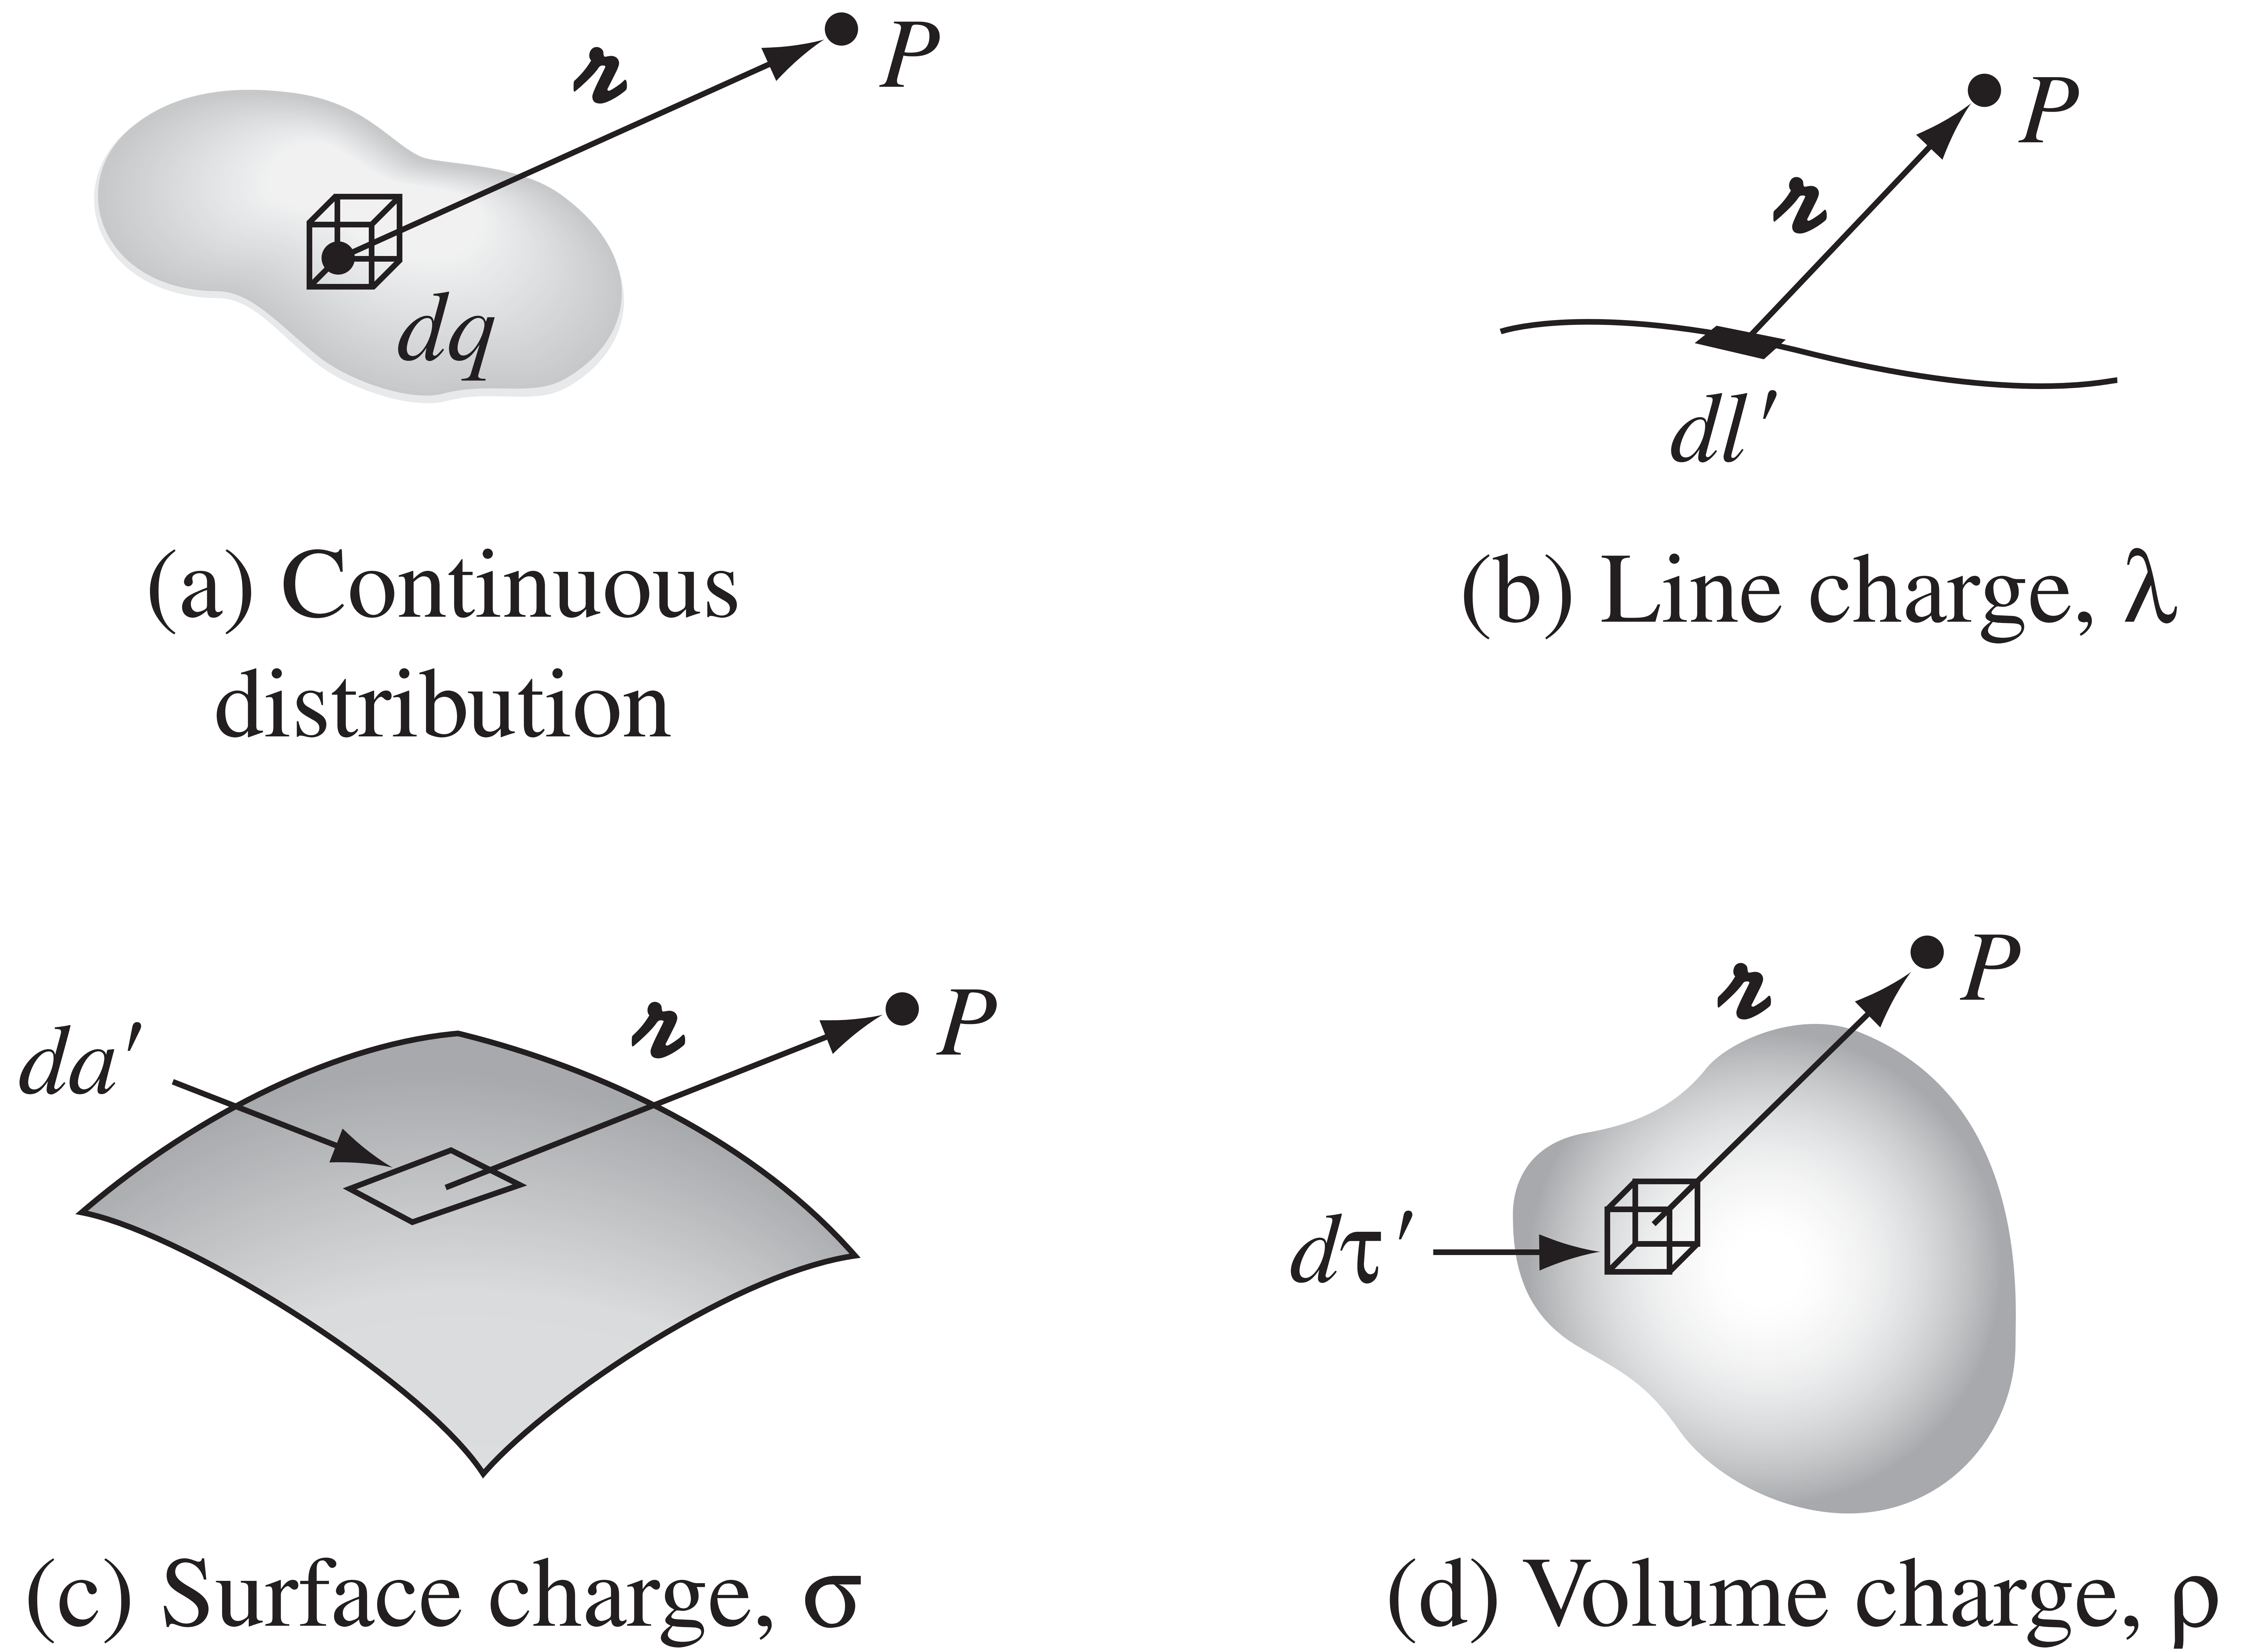
\includegraphics[height=5cm]{../Rss/Electromagnetism/Electrostatics/ChargeDis.png}
    \caption*{Charge Distribution}
\end{figure*}
Thus the electric field of a line charge is
\begin{equation*}
    \mathbf{E}=\frac{1}{4\pi \epsilon_0}\int\frac{\lambda(\mathbf{r'})}{\rcurs_i^2}\hrcurs\;dl'
\end{equation*}
for a surface charge
\begin{equation*}
    \mathbf{E}=\frac{1}{4\pi \epsilon_0}\int\frac{\sigma(\mathbf{r'})}{\rcurs_i^2}\hrcurs\;da'
\end{equation*}
and for a volume charge
\begin{equation*}
    \mathbf{E}=\frac{1}{4\pi \epsilon_0}\int\frac{\rho(\mathbf{r'})}{\rcurs_i^2}\hrcurs\;d\tau'
\end{equation*}

\subsubsection*{Gauss's law.} 
The flux of \textbf{E} through a surface S 
\begin{equation*}
    \Phi_E \equiv \int_{S} \mathbf{E}\cdot d\mathbf{a}
\end{equation*}
is a measure of the “number of field lines” passing through S. The flux through any closed surface is a measure of the
total charge inside. This is the essence of Gauss's law. 
\begin{equation*}
    \oint \mathbf{E}\cdot d\mathbf{a}=\frac{1}{\epsilon_0}Q_{enc}
\end{equation*}
applying the divergence theorem
\begin{equation*}
    \int_{\mathcal{V}}(\nabla \cdot \mathbf{E})\;d\tau=\int_{\mathcal{V}} \frac{\rho}{\epsilon_0}\;d\tau
\end{equation*}
And since this holds for any volume, the integrands must be equal
\begin{equation*}
    \nabla \cdot \mathbf{E}=\frac{1}{\epsilon_0}\rho
\end{equation*}

\subsubsection*{Divergence of E.} Gauss's law state the divergence of \textbf{E} in differential form
\begin{equation*}
    \nabla \cdot \mathbf{E}=\frac{1}{\epsilon_0}\rho
\end{equation*}

\subsubsection*{Curl of E.} The integral of \textbf{E} around a closed path is zero 
\begin{equation*}
    \oint \mathbf{E} \cdot d\mathbf{l}  =0
\end{equation*}
and hence, applying Stokes' theorem
\begin{equation*}
    \nabla \times \mathbf{E}  =0
\end{equation*}


\subsection*{Potential}
\subsubsection*{Introduction to Potential.} Because the line integral of \textbf{E} is independent of path, we can define a function
\begin{equation*}
    V(r)\equiv -\int_{\mathcal{O}}^{r} \mathbf{E}(\mathbf{r'})\cdot d\mathbf{l'}
\end{equation*}
The potential difference between two points a and b is
\begin{equation*}
    V (b) - V (a)= -\int_{a}^{b} \mathbf{E}(\mathbf{r'})\cdot d\mathbf{l'}
\end{equation*}
Applying fundamental theorem for gradients, we get
\begin{equation*}
    \mathbf{E} =-\nabla V
\end{equation*}
Electric field \textbf{E} will point from high potential to low potential.

\subsubsection*{Poisson's Equation and Laplace's Equation}
Poisson's Equation state the divergence of E in terms of volume. 
Since $   \mathbf{E} =-\nabla V$, divergence of E in terms of V
\begin{equation*}
    \nabla^2 V=-\frac{\rho}{\epsilon_0}
\end{equation*}
This is known as Poisson's equation. In regions where there is no charge, so
$\rho = 0$, Poisson's equation reduces to Laplace's equation:
\begin{equation*}
    \nabla^2 V=0
\end{equation*}

\subsubsection*{The Potential of a Localized Charge Distribution.}
In general, the potential of a collection of charges is
\begin{equation*}
    V(\mathbf{r})=\frac{1}{4\pi \epsilon_0} \sum_{i=1}^{n}\frac{q_i}{\rcurs_i}
\end{equation*}
or, for a continuous distribution
\begin{equation*}
    V(\mathbf{r})=\frac{1}{4\pi \epsilon_0} \int\frac{1}{\rcurs}dq
\end{equation*}
and, for a volume charge, it's
\begin{equation*}
    V(\mathbf{r})=\frac{1}{4\pi \epsilon_0} \int\frac{\rho(\mathbf{r'})}{\rcurs}d\tau'
\end{equation*}

\subsubsection*{Boundary Conditions.}
We have, in the course of our discussion, discussed the three
fundamental quantities of electrostatics: $\rho$, $\mathbf{E}$, and V and derived all six formulas interrelating  them. 

\begin{figure*}[b]
    \centering
    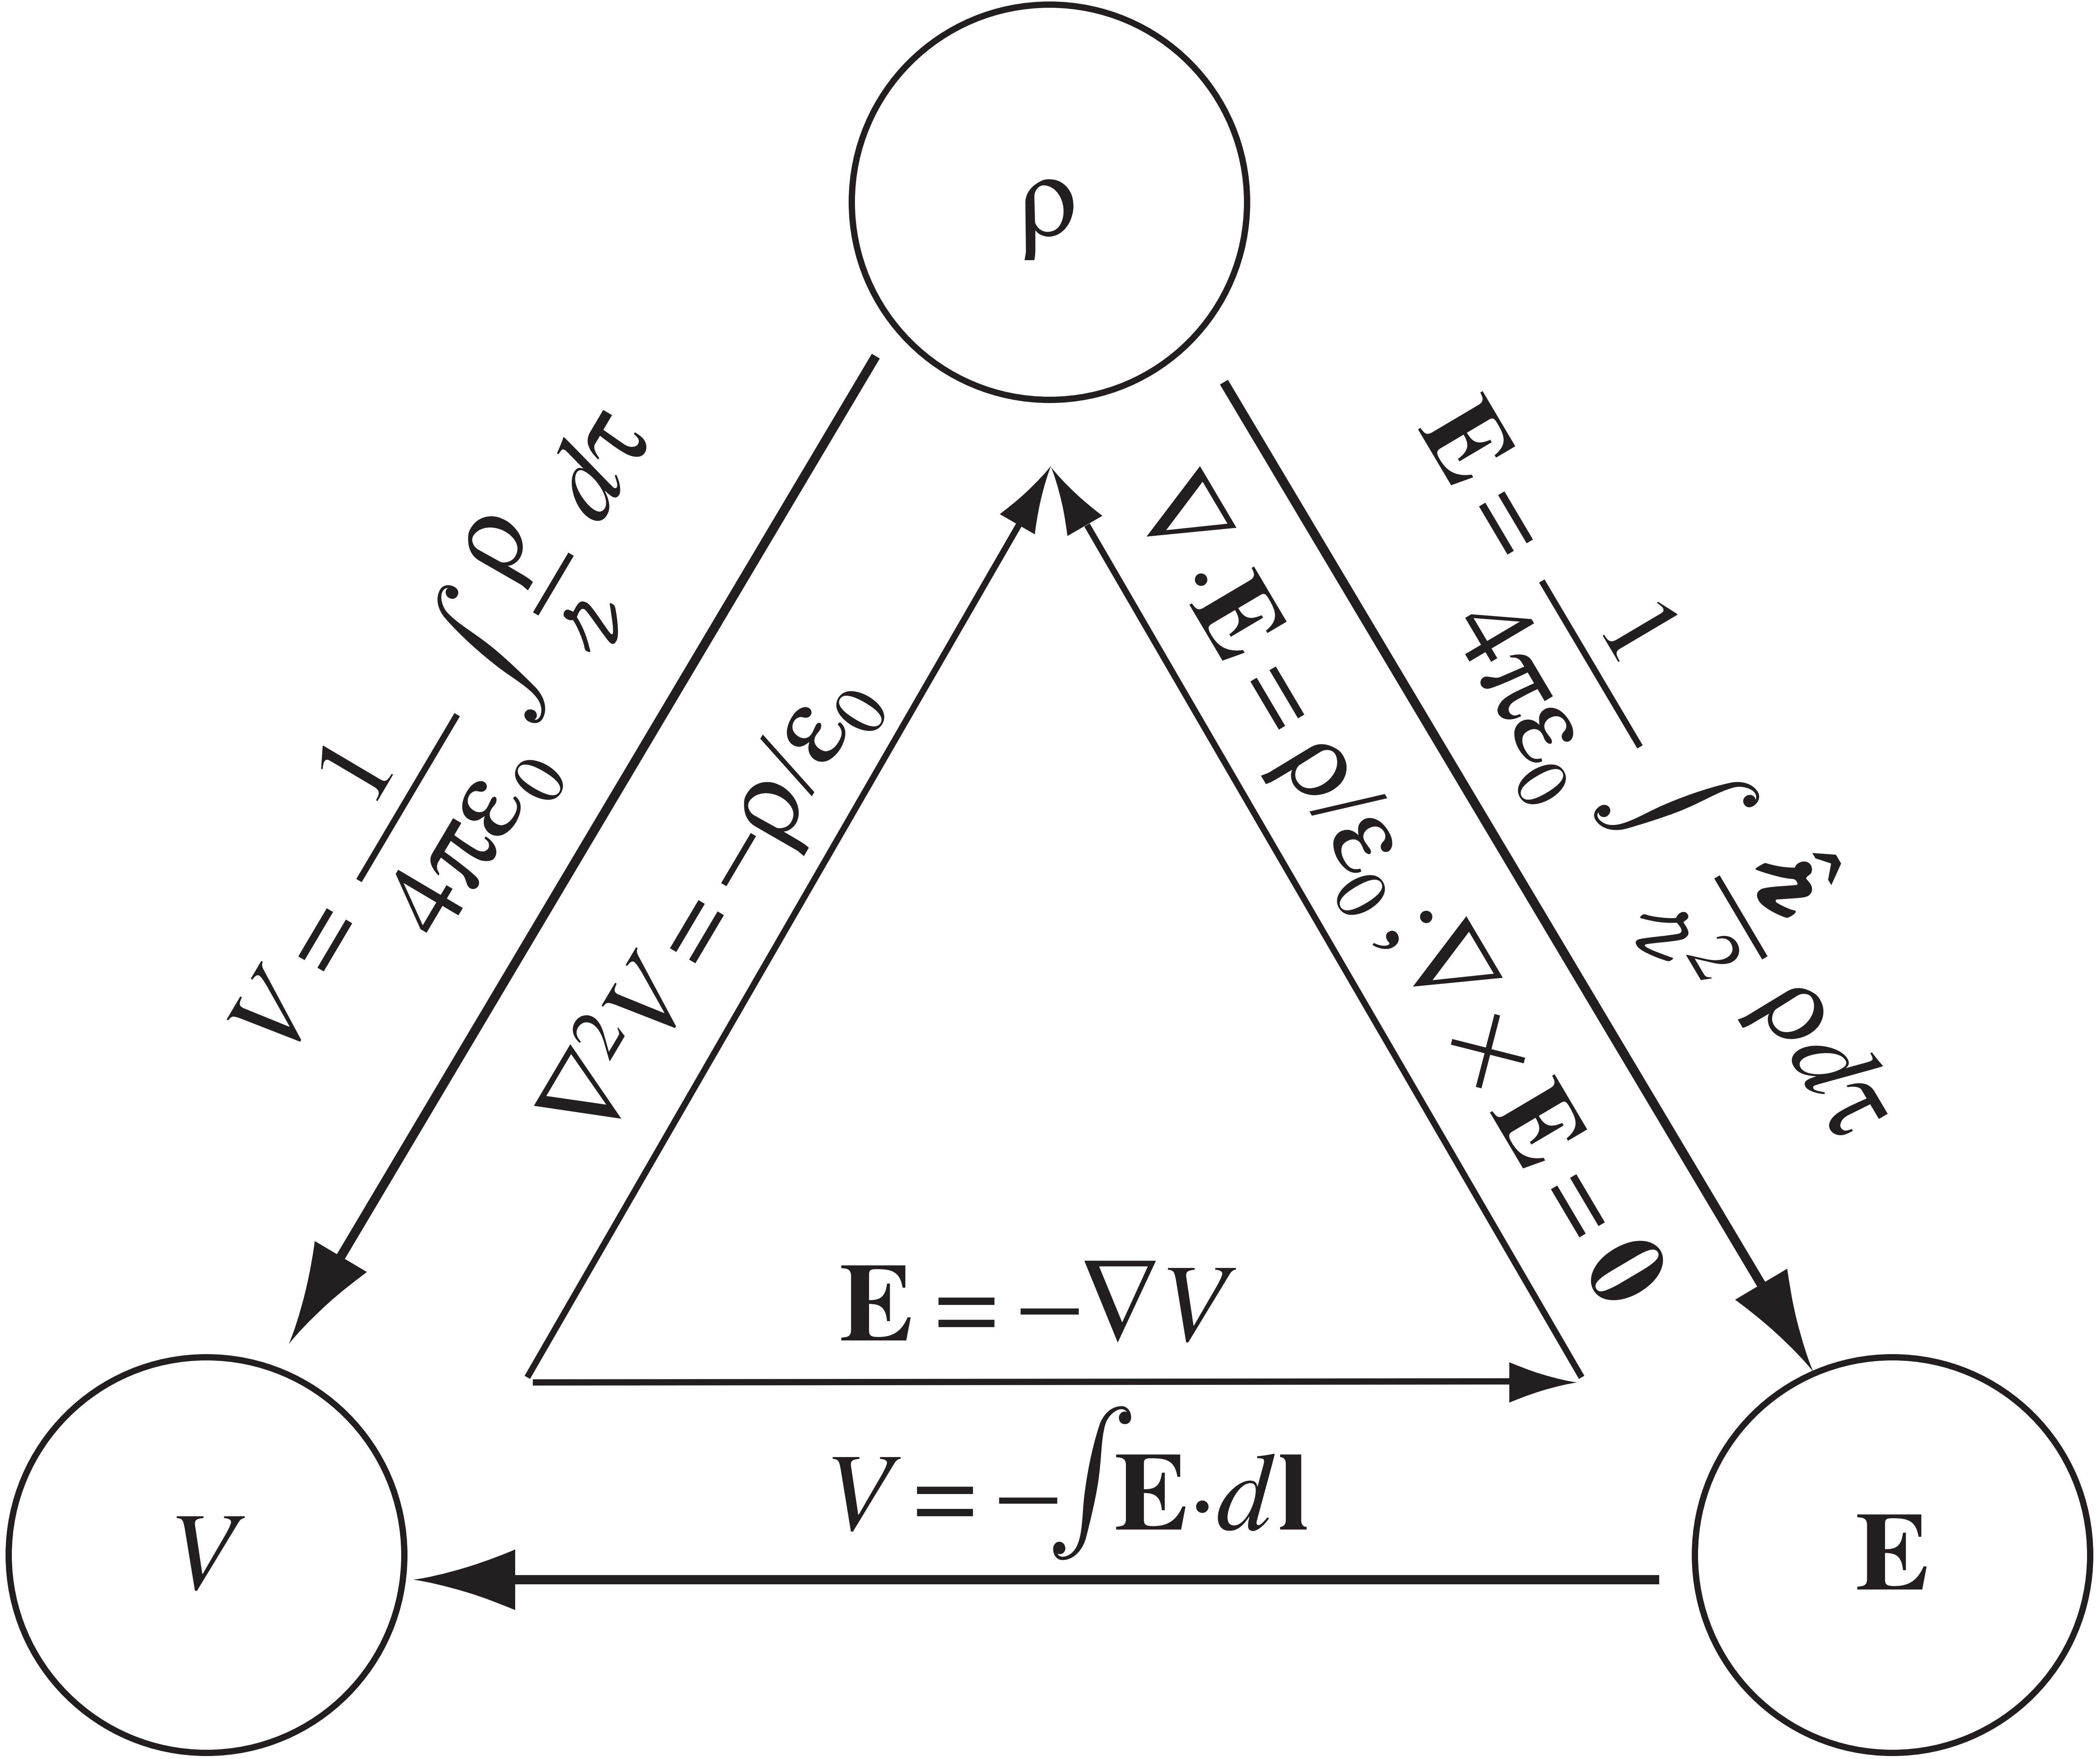
\includegraphics[height=5cm]{../Rss/Electromagnetism/Electrostatics/ElecstatHolyTrinity.png}
    \caption*{Figure: Electrostatics Holy Trinity}
\end{figure*}

Electric field always undergoes a discontinuity
when you cross a surface charge $\sigma$
The normal component of \textbf{E} is discontinuous by an amount $\sigma/\epsilon_0$ at any boundary.
In particular, where there is no surface charge, perpendicular electric $E^\bot$ field is continuous, as for instance at the
surface of a uniformly charged solid sphere.
\begin{equation*}
    E^\bot_{\text{above}}-E^\bot_{\text{below}}=\frac{\sigma}{\epsilon_0}
\end{equation*}
The tangential component of \textbf{E} ($E^{||}$), by contrast, is always continuous.
\begin{equation*}
    E^{||}_{\text{above}}=E^{||}_{\text{below}}
\end{equation*}
The equation then can be summarized by
\begin{equation*}
    \mathbf{E}_{\text{above}}- \mathbf{E}_{\text{below}}=\frac{\sigma}{\epsilon_0}\mathbf{\hat{n}}
\end{equation*}

In terms of potential,
\begin{equation*}
    \nabla V_{\text{above}}-\nabla V_{\text{below}}=-\frac{\sigma}{\epsilon_0}\mathbf{\hat{n}}
\end{equation*}
or
\begin{equation*}
    \frac{\partial V_{\text{above}}}{\partial n}- \frac{\partial V_{\text{below}}}{\partial n}=-\frac{\sigma}{\epsilon_0}
\end{equation*}
where
\begin{equation*}
    \frac{\partial V}{\partial n}=\nabla V\cdot \mathbf{\hat{n}}
\end{equation*}
denotes the normal derivative of V (that is, the rate of change in the direction
perpendicular to the surface). Meanwhile, potential is continuous across any boundary $V_{\text{above}}=V_{\text{below}}$

\subsection*{Work}
\subsubsection*{The Work It Takes to Move a Charge.}
The work you do to move a test charge Q from point a to point b is
\begin{equation*}
    W=\int_{a}^{b} \mathbf{F}\cdot d\mathbf{l}=-Q\int_{a}^{b}  \mathbf{E}\cdot d\mathbf{l}=Q[V(\mathbf{b})-V(\mathbf{a})]
\end{equation*}
Work also defined as the difference in potential energy $U$ of system
\begin{equation*}
    W=\Delta U
\end{equation*}
If you have set the reference point (point a) at infinity, therefore
\begin{equation*}
    W=QV(\mathbf{r})
\end{equation*}
In this sense, potential $V$ is potential energy $W$ (the work it takes to create the system) per unit charge $Q$, just as the field is the force per unit charge ($\mathbf{E}=\mathbf{F}/Q$).

\subsubsection*{The Energy of a Point Charge Distribution.}
The work it would take to assemble an entire collection of point charges is 
\begin{equation*}
    W=\frac{1}{2}\sum_{i=1}^{n}q_i\biggl(\sum_{j\neq i}^{n}\frac{1}{4\pi \epsilon_0}\frac{q_j}{\rcurs_{ij}}\biggr)=\frac{1}{2}\sum_{i=1}^{n}q_iV(\mathbf{r}_i)
\end{equation*}
where $V(\mathbf{r}_i)$ is potential at point $\mathbf{r}_i$
\begin{figure*}[b]
    \centering
    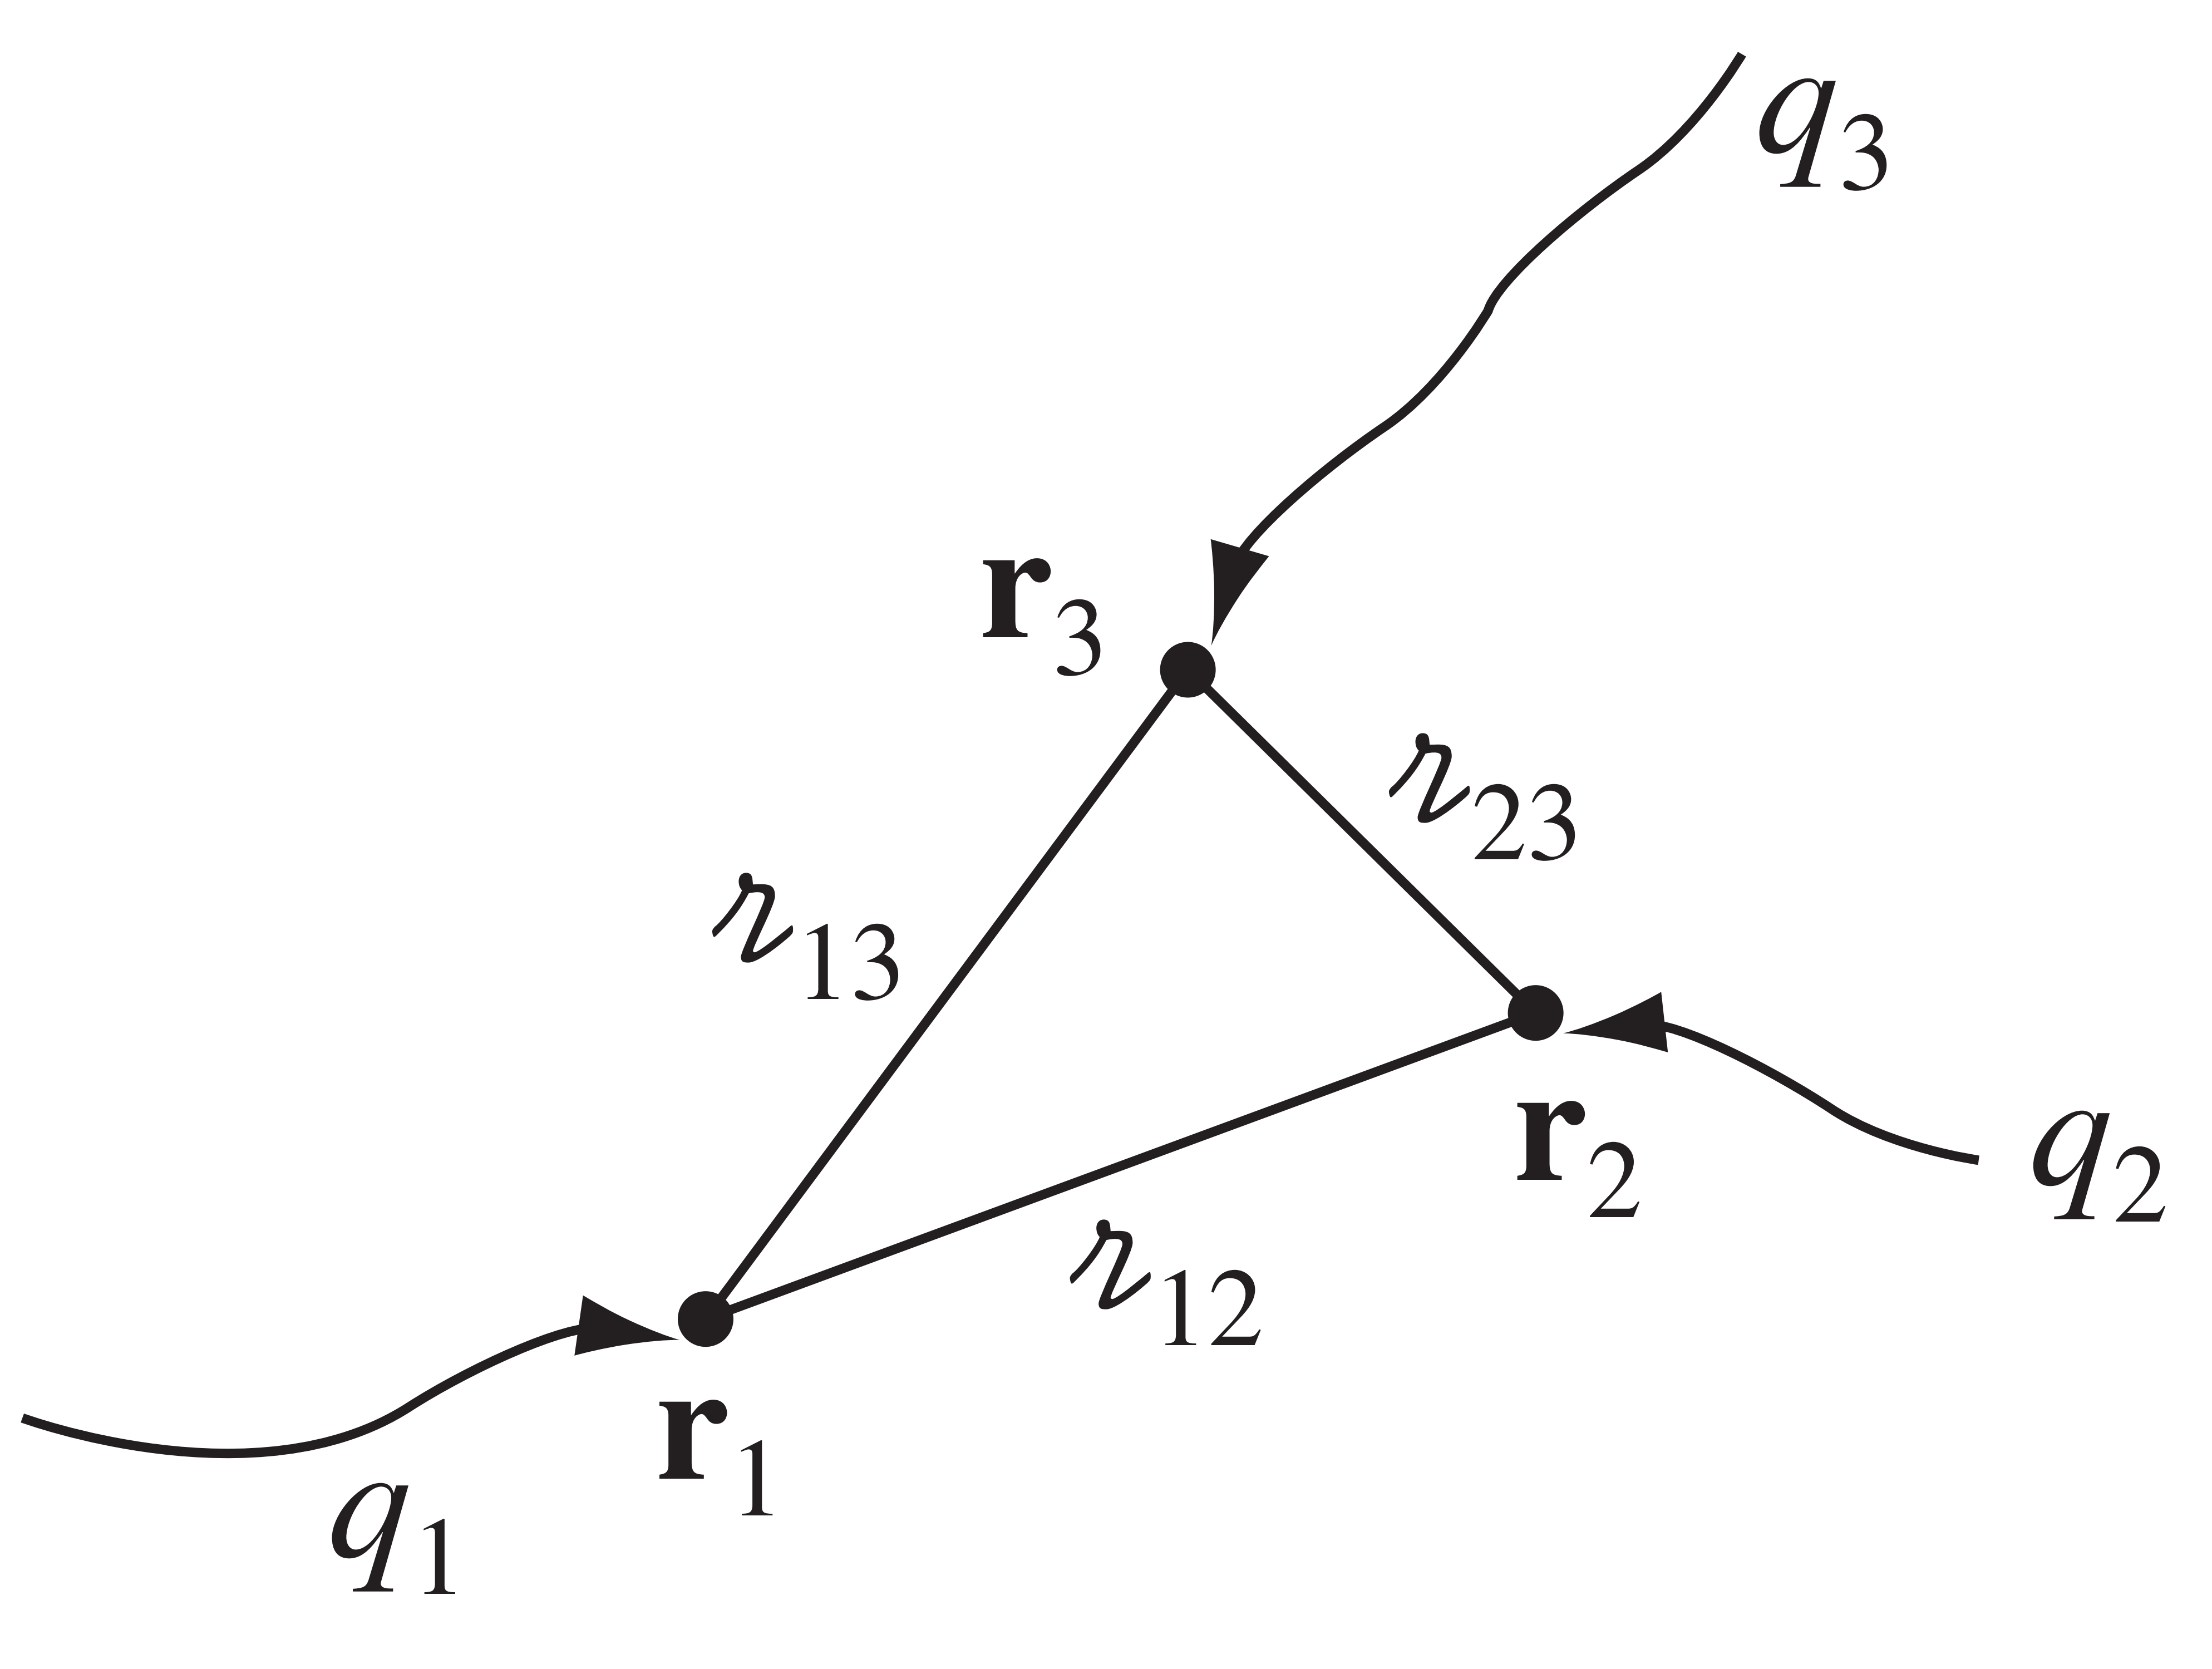
\includegraphics[height=5cm]{../Rss/Electromagnetism/Electrostatics/WorkPointChar.png}
    \caption*{Point Charges}
\end{figure*}
\subsubsection*{The Energy of a Continuous Charge Distribution.} For a volume charge density,
\begin{equation*}
    W=\frac{1}{2}\int\rho V\;d\tau
\end{equation*}
which can be written using Gauss's law and integration by parts as
\begin{equation*}
    W=\frac{\epsilon_0}{2}\Biggl(\int_{V}E^2\;d\tau+ \oint V\mathbf{E}\cdot d\mathbf{a}\Biggr)
\end{equation*}
Integration can be done over whatever volume you use (as long as it encloses all the charge), but the contribution from the volume integral goes up, and that of the surface integral goes down, as you take larger and larger volumes. In particular, why not integrate over all space? Thus,
\begin{equation*}
    W=\frac{\epsilon_0}{2}\int E^2\;d\tau\quad\text{Over all Space}
\end{equation*}

\subsubsection*{Where is the energy stored?} In the context of radiation theory it is useful (and in general relativity it is essential) to regard the energy as stored in the field, with a density
\begin{equation*}
    U=\frac{\epsilon_0 }{2}E^2
\end{equation*}
But in electrostatics one could just as well say it is stored in the charge, with a density $\frac{1}{2}\rho V$.

\subsection*{Conductor}
\subsubsection*{Basic Properties.}
A perfect conductor would contain an unlimited supply of free charges. From this definition, the basic electrostatic properties of ideal conductors immediately follow
\begin{enumerate}
    \item \textbf{E} = 0 inside a conductor
    \item $\rho$ = 0 inside a conductor
    \item Any net charge resides on the surface
    \item A conductor is an equipotential
    \item \textbf{E} is perpendicular to the surface, just outside a conductor
\end{enumerate}

\subsubsection*{Surface Charge and the Force on a Conductor.} 
Because the field inside a conductor is zero, 
the field immediately outside is
\begin{equation*}
    \mathbf{E}=\frac{\sigma}{\epsilon_0}\mathbf{\hat{n}}
\end{equation*}
Applying boundary condition, the surface charge on a conductor in
terms of potential is
\begin{equation*}
    \sigma=-\epsilon_0\frac{\partial V}{\partial n}
\end{equation*}

In the presence of an electric field, a surface charge will experience a force; the force per unit area, \textbf{f}, is $\sigma\mathbf{E}$
\begin{equation*}
    \mathbf{f}=\sigma\mathbf{E}_{\text{average}}=\frac{1}{2}\sigma(\mathbf{E}_{\text{above}}-\mathbf{E}_{\text{below}})
\end{equation*}
In the case of a conductor, the field is zero inside. Therefore,
    \begin{equation*}
        \mathbf{f}=\frac{1}{2\epsilon_0}\sigma^2\mathbf{\hat{n}}
    \end{equation*} 
This amounts to an outward electrostatic pressure on the surface, tending to draw the conductor into the field, regardless of the sign of $\sigma$. Expressing the pressure in terms of the field just outside the surface
\begin{equation*}
    P=\frac{\epsilon_0}{2}E^2
\end{equation*}

\subsubsection*{Capacitor.}
Since \textbf{E} is proportional to Q, so also is V. The constant of proportionality is called the capacitance of the arrangement:
\begin{equation*}
    C\equiv \frac{Q}{V}
\end{equation*}
\end{document}